\documentclass{article}
\usepackage[margin=1in]{geometry}
\usepackage{amsmath,amsfonts}
\usepackage{parskip}
\usepackage{graphicx}
\usepackage{hyperref}
\setlength{\parindent}{0pt}

\begin{document}

\title{Proposed Architecture for the K-Square Project Onboarding Agent}
\author{Alberto Espinosa \\ KSquare Group}
\date{1 August 2025}
\maketitle

\begin{abstract}
The K-Square Project Onboarding Agent aims to streamline the onboarding of programme execution teams by automating data aggregation and insight generation. This document proposes a robust architecture to support this goal, detailing agentic separation, system layers, and recommended technologies. The architecture leverages LangGraph for agent orchestration and Ollama for local language model inference, complemented by additional tools to ensure scalability, privacy, and efficiency. Four diagrams illustrate the system’s design, providing visual clarity on agent interactions, data flow, architecture, and high-level workflow.
\end{abstract}

\section{Introduction}
The K-Square Project Onboarding Agent addresses the challenge of manual onboarding by providing execution teams with rapid access to client profiles, domain knowledge, and project insights. A well-designed architecture is essential to ensure seamless data processing, agent coordination, and user interaction. This proposal outlines a layered architecture with distinct agents, focusing on technical feasibility and alignment with enterprise workflows.

\section{Architecture Overview}
The architecture is structured into five layers: Data, Agent, Processing, UI, and Orchestration. Three specialised agents---Deep Dive, Project Intelligence, and Meetings---operate within the Agent Layer to perform research, aggregation, and meeting analysis tasks. The system integrates internal data from repositories (e.g., SharePoint) and external data from web sources, delivering actionable outputs through a user-friendly interface. LangGraph orchestrates agent workflows, while Ollama powers local language model inference for privacy-sensitive tasks.

\section{Agentic Separation}
The system employs three distinct agents, each with specific roles, inputs, and outputs:

\subsection{Deep Dive Agent}
The Deep Dive Agent conducts comprehensive research to gather client-specific and industry-relevant information. It queries internal repositories (e.g., SharePoint folders organised by industry and client) and external web sources. Inputs include project identifiers and client names; outputs include ranked documents and summaries, validated by human feedback to ensure relevance.

\subsection{Project Intelligence Agent}
The Project Intelligence Agent aggregates outputs from other agents to produce a consolidated dashboard. It processes data from the Deep Dive and Meetings Agents, generating summaries, recommendations, and actionable outputs such as statements of work or presentations. Its role is to synthesise information into a format suitable for execution teams.

\subsection{Meetings Agent}
The Meetings Agent analyses meeting data, such as audio recordings or transcripts from Microsoft Teams, to extract action items, sentiment, and potential scope expansions. It employs speech-to-text and natural language processing techniques to provide insights that enhance future client interactions.

\section{Layer Descriptions}
The architecture comprises five layers, each addressing a critical aspect of the system:

\subsection{Data Layer}
The Data Layer manages the ingestion, storage, and preprocessing of internal and external data. Internal data, such as statements of work and discovery documents, are retrieved from SharePoint via the Microsoft Graph API. External data, including public records and industry trends, are collected through web crawling. A vector database (e.g., Pinecone) stores document embeddings for efficient semantic search. Preprocessing involves text extraction from documents using optical character recognition (e.g., Tesseract) and chunking with natural language processing libraries (e.g., SpaCy).

\subsection{Agent Layer}
The Agent Layer hosts the Deep Dive, Project Intelligence, and Meetings Agents, orchestrated by LangGraph. LangGraph’s graph-based framework defines workflows where agents exchange data (e.g., Deep Dive outputs feed Project Intelligence). Ollama runs local large language models (e.g., LLaMA 3) for processing internal data, ensuring privacy. External data processing may leverage cloud-based models (e.g., OpenAI) for enhanced performance.

\subsection{Processing Layer}
The Processing Layer handles language model inference, vector search, and feedback integration. Large language models are fine-tuned on internal data using techniques like LoRA to improve domain-specific accuracy. Vector search, powered by Pinecone or Weaviate, enables rapid retrieval of relevant documents. A feedback mechanism collects user validations (e.g., relevance scores) to retrain models periodically, enhancing system performance over time.

\subsection{UI Layer}
The UI Layer provides a React-based dashboard for user interaction, featuring tabs for client profiles, domain knowledge, and meeting insights. Users can validate agent outputs (e.g., via checkboxes) and view visualisations (e.g., engagement metrics) using Chart.js. The dashboard connects to the backend via a REST API (e.g., FastAPI) to fetch and submit data.

\subsection{Orchestration Layer}
The Orchestration Layer, powered by LangGraph, manages agent workflows and system monitoring. Workflows are defined as graphs, with nodes representing agent tasks and edges denoting data flow. Monitoring tools, such as Prometheus and Grafana, track agent performance and language model accuracy, ensuring reliability and scalability.

\section{Proposed Technologies}
The following technologies are recommended, with justifications and alternatives:

\subsection{LangGraph}
LangGraph is proposed for orchestrating agent workflows due to its flexibility in managing dynamic task dependencies. It supports context retention, enabling seamless data exchange between agents. However, its complexity may require experienced developers. CrewAI, a simpler alternative, is suitable for prototyping but lacks LangGraph’s scalability for production.

\subsection{Ollama}
Ollama is recommended for local language model inference, ensuring data privacy for internal documents. It supports models like LLaMA 3, suitable for summarisation and insight generation. Its limitation is performance with large-scale inference, necessitating cloud-based models (e.g., OpenAI, Google Gemini) for external data processing.

\subsection{Supporting Technologies}
\begin{itemize}
    \item \textbf{Pinecone}: A vector database for semantic search, offering scalability and speed. Weaviate is a viable alternative with open-source options.
    \item \textbf{Whisper}: OpenAI’s speech-to-text model for transcribing meeting recordings, with high accuracy across languages.
    \item \textbf{FastAPI}: A lightweight framework for building REST APIs to connect the UI and backend.
    \item \textbf{React}: A robust library for building an interactive dashboard, with Material-UI for styling.
    \item \textbf{Prometheus and Grafana}: Monitoring tools to track system performance and ensure reliability.
\end{itemize}

\section{System Diagrams}
The system’s design is illustrated through four diagrams, embedded below with detailed explanations. These diagrams clarify agent interactions, data flow, architectural layers, and the high-level workflow.

\subsection{Agents Interaction Diagram}
\begin{figure}[h]
    \centering
    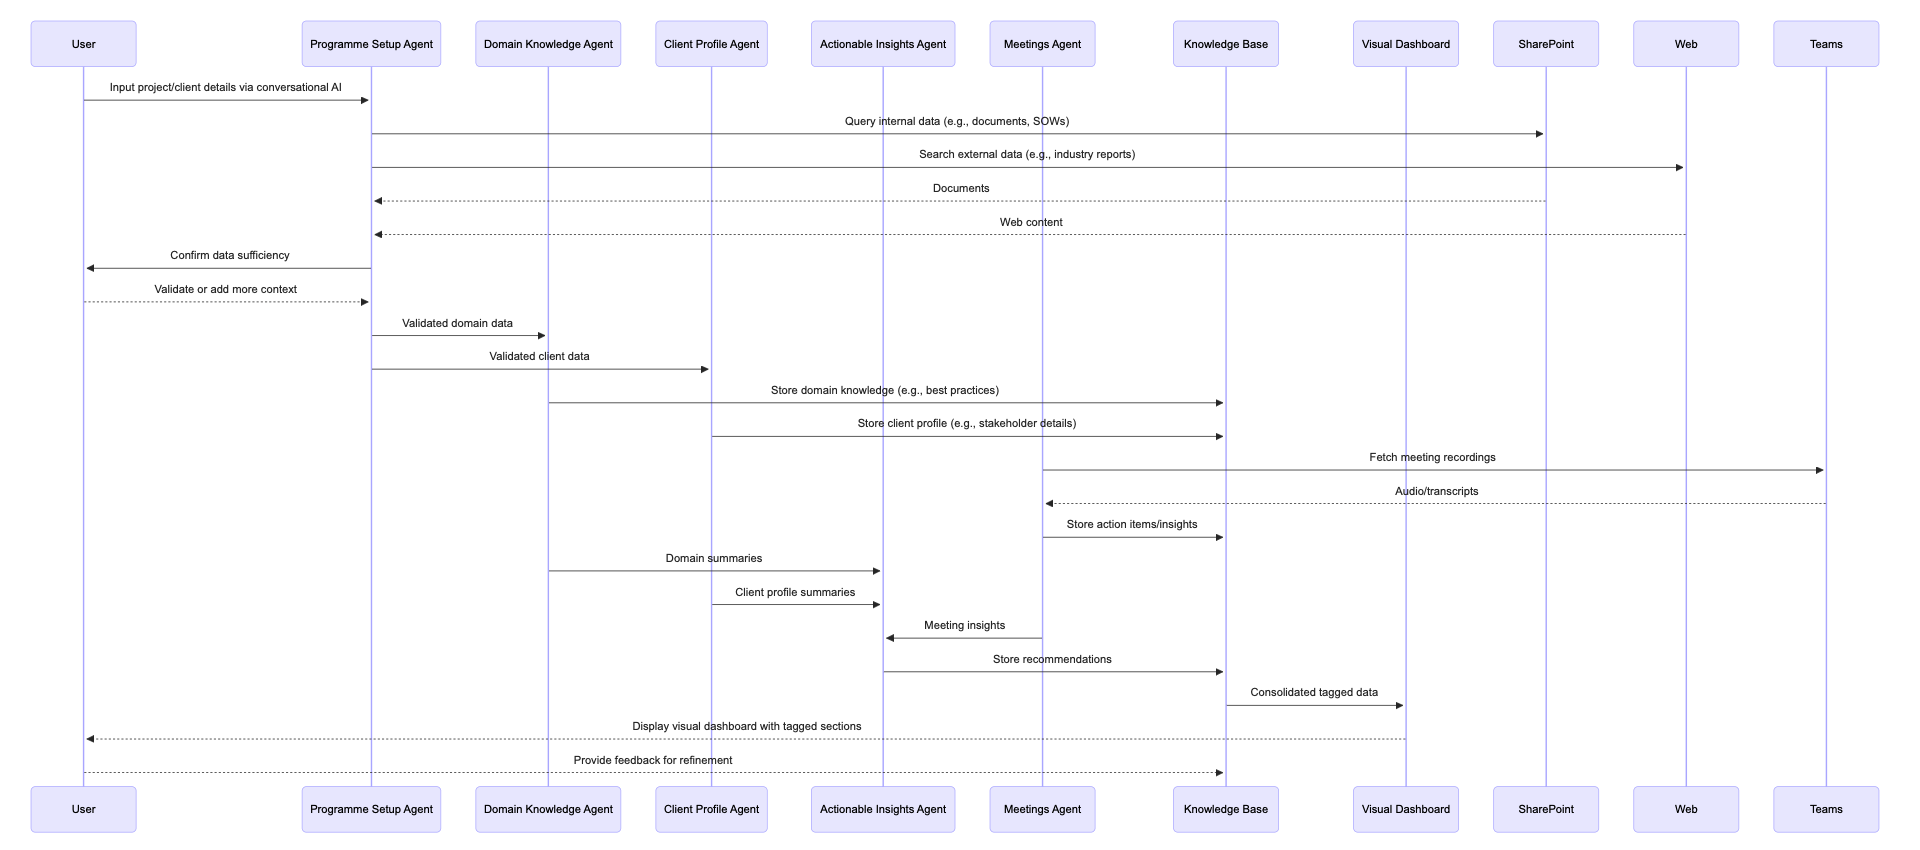
\includegraphics[width=1\textwidth]{/Users/albertohernandez/Documents/projects/KS-onboarding/doc/images/agents_interaction.png}
    \caption{Agents Interaction Diagram.}
    \label{fig:agents_interaction}
\end{figure}
Figure \ref{fig:agents_interaction} is a sequence diagram illustrating the interactions between the Deep Dive, Project Intelligence, and Meetings Agents. The process begins with a user providing project or client details to the Deep Dive Agent, which queries SharePoint and web sources for relevant data. The agent presents results for user validation, then passes validated summaries to the Project Intelligence Agent. Concurrently, the Meetings Agent retrieves audio or transcripts from Microsoft Teams, extracting insights such as action items and sentiment. These insights are sent to the Project Intelligence Agent, which consolidates all data into a dashboard displayed to the user. This diagram highlights the collaborative nature of the agents and the role of human validation in ensuring accuracy.

\subsection{Data Flow Diagram}
\begin{figure}[h]
    \centering
    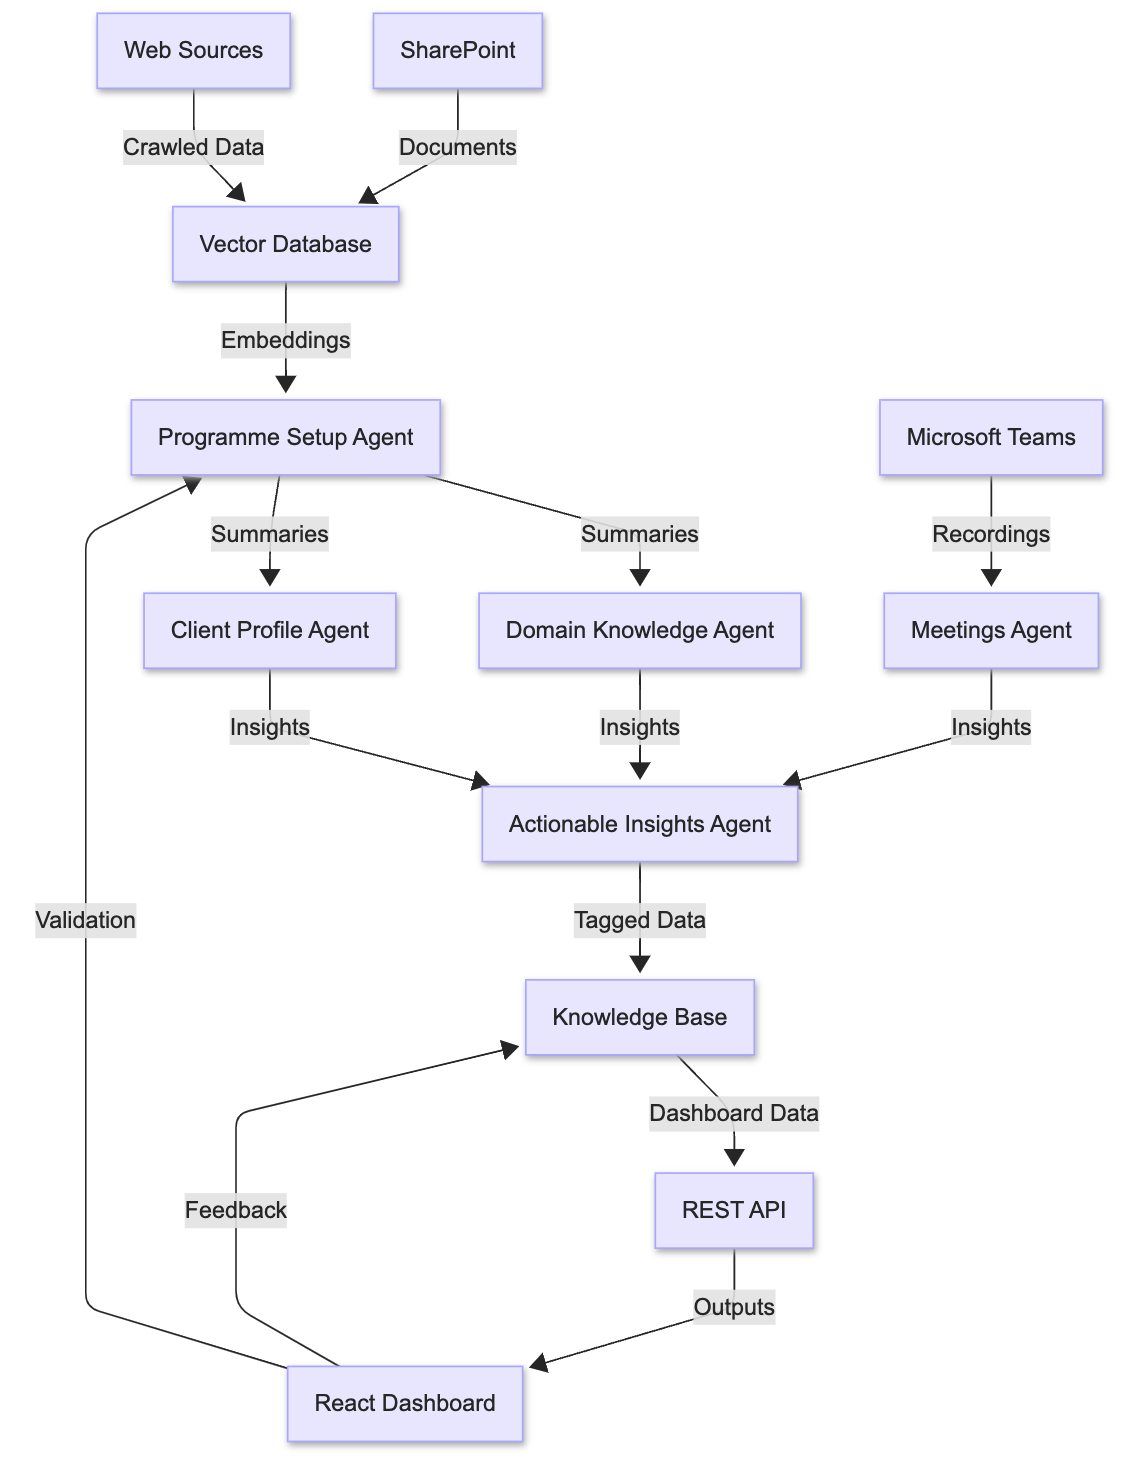
\includegraphics[width=0.8\textwidth]{/Users/albertohernandez/Documents/projects/KS-onboarding/doc/images/data_flow.png}
    \caption{Data Flow Diagram.}
    \label{fig:data_flow}
\end{figure}
Figure \ref{fig:data_flow} depicts the flow of data through the system. Internal documents from SharePoint and external web content are ingested into a vector database for semantic search. The Deep Dive Agent retrieves and processes this data, producing summaries that are validated by the user. The Meetings Agent processes Microsoft Teams recordings, extracting insights that feed into the Project Intelligence Agent. The Project Intelligence Agent synthesises these inputs into dashboard data, which is served to the React dashboard via a REST API. User feedback and validations loop back to refine agent outputs, illustrating the system’s closed-loop design.

\subsection{Architecture Diagram}
\begin{figure}[h]
    \centering
    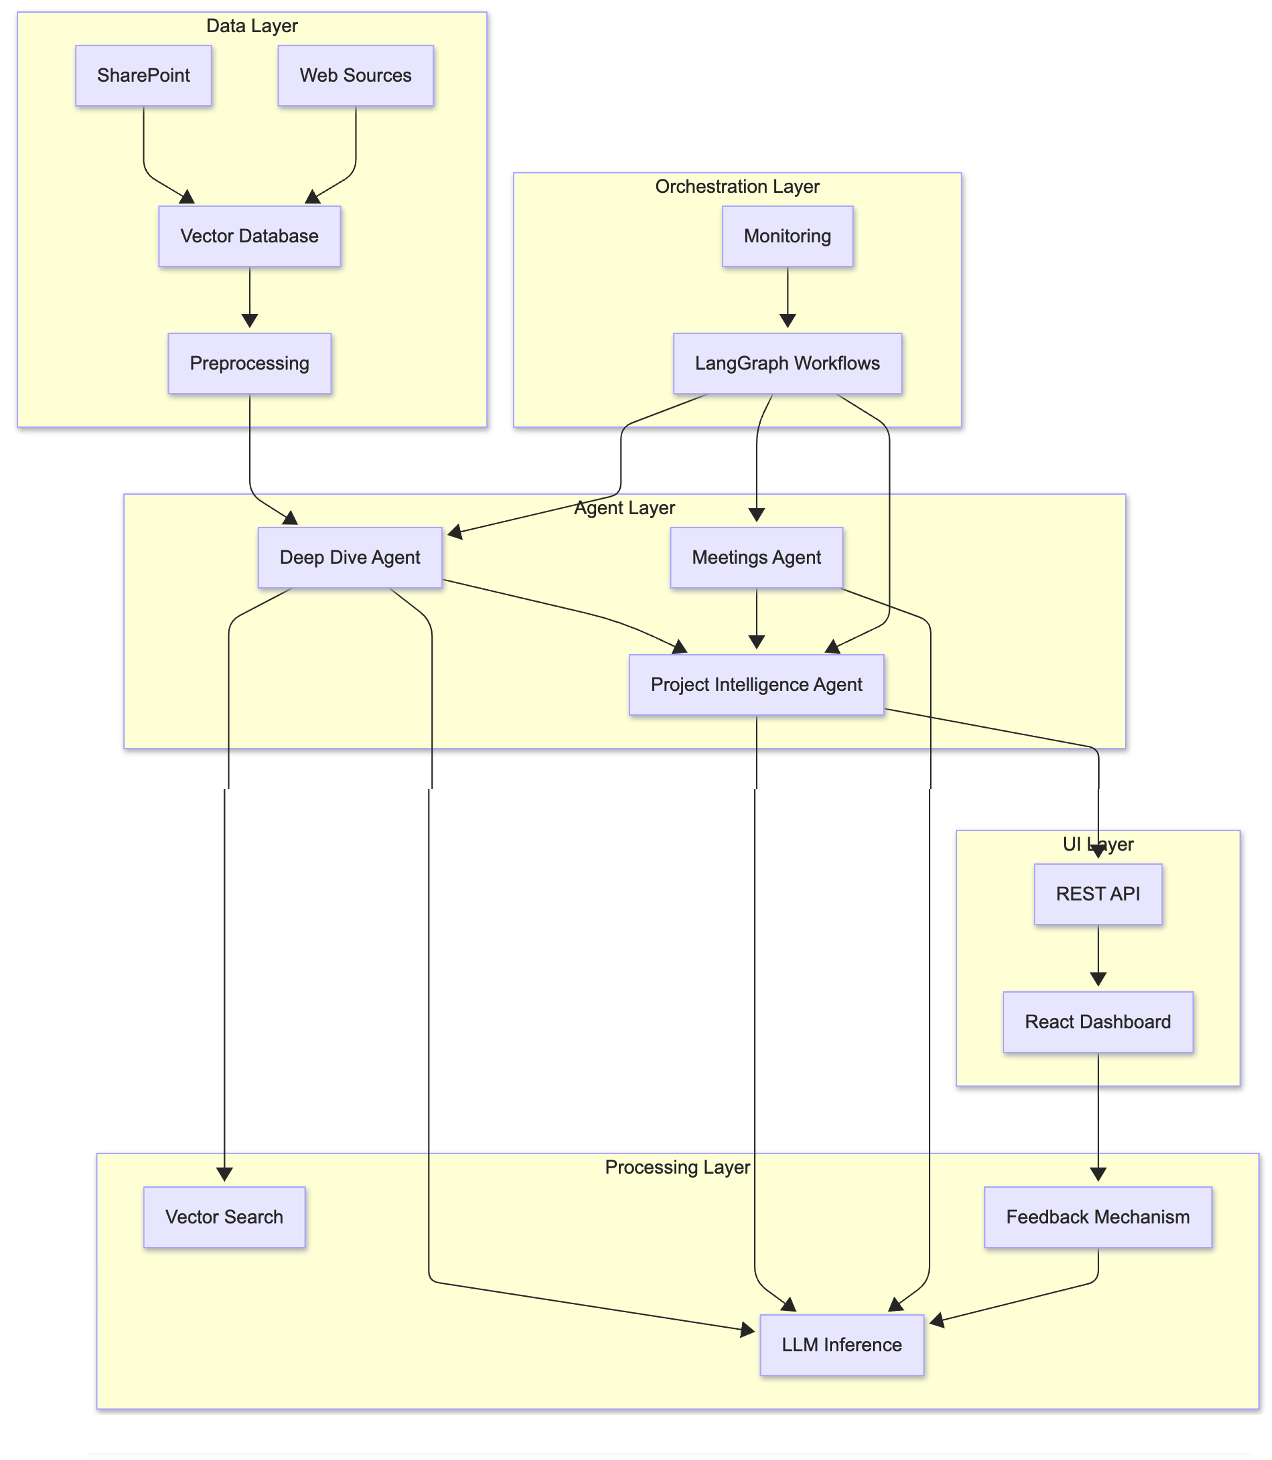
\includegraphics[width=1\textwidth]{/Users/albertohernandez/Documents/projects/KS-onboarding/doc/images/architecture.png}
    \caption{Architecture Diagram.}
    \label{fig:architecture}
\end{figure}
Figure \ref{fig:architecture} outlines the system’s five layers: Data, Agent, Processing, UI, and Orchestration. The Data Layer includes SharePoint, web sources, a vector database, and preprocessing components. The Agent Layer hosts the Deep Dive, Project Intelligence, and Meetings Agents, coordinated by LangGraph. The Processing Layer manages language model inference, vector search, and feedback integration. The UI Layer delivers a React-based dashboard via a REST API. The Orchestration Layer, powered by LangGraph, defines workflows and monitors performance with Prometheus and Grafana. This diagram provides a comprehensive view of the system’s technical structure.

\subsection{High-Level Overview Diagram}
\begin{figure}[h]
    \centering
    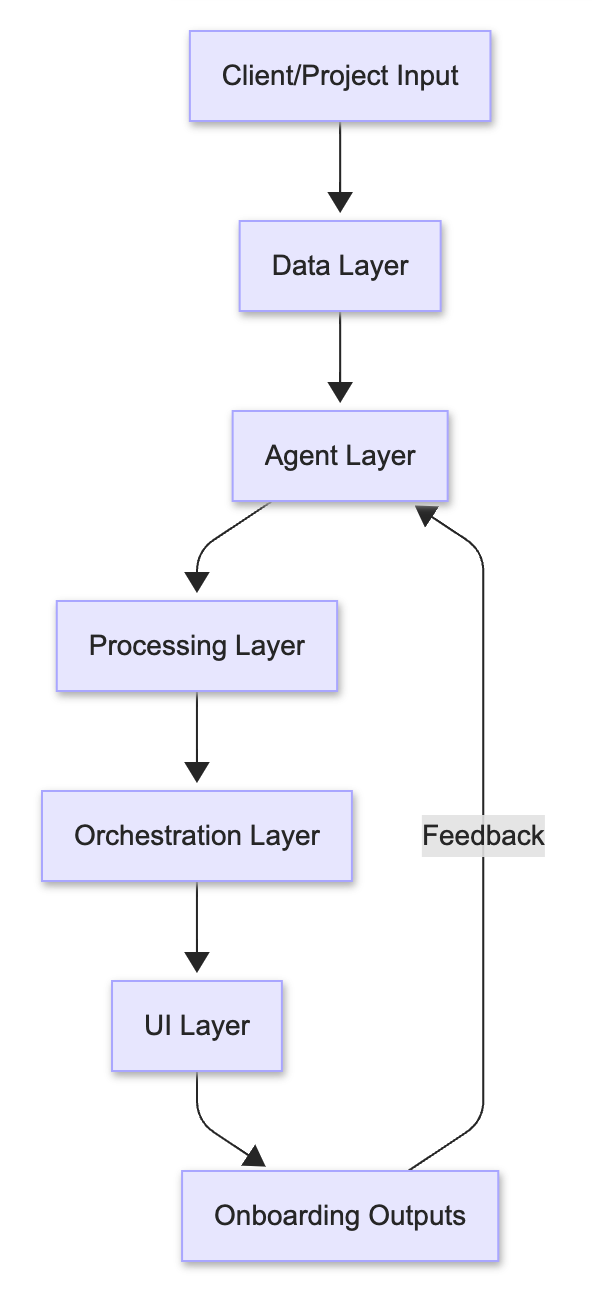
\includegraphics[width=0.5\textwidth]{/Users/albertohernandez/Documents/projects/KS-onboarding/doc/images/overview.png}
    \caption{High-Level Overview Diagram.}
    \label{fig:overview}
\end{figure}
Figure \ref{fig:overview} presents a simplified view of the system’s end-to-end workflow. Client and project inputs are processed through the Data, Agent, Processing, and Orchestration Layers, culminating in onboarding outputs displayed via the UI Layer. Feedback loops back to the Agent Layer, enabling continuous improvement. This diagram encapsulates the system’s purpose: to transform raw inputs into actionable onboarding insights efficiently.

\section{Suggested Additional Features}
The Meetings Agent, as outlined in the Agentic Separation section, utilises sentiment analysis to extract insights from meeting data, offering a general indication of the tone and opinions expressed during client interactions. To enhance this capability, a novel approach proposed by \textbf{Alberto Espinosa} introduces a formal dynamical measurement of opinion change based on semantics and complexity \cite{espinosa2025}. This research, detailed at \href{https://arxiv.org/abs/2505.02581}{https://arxiv.org/abs/2505.02581}, develops a change-of-opinion attack test using perturbation and intervention analysis to study how humans and agents influence conversational dynamics. The study posits that tracking shifts in semantics, sentiment, and topics provides a more nuanced understanding of interactions, which is particularly relevant for the Meetings Agent. By integrating this measurement, the system can better assess how client perspectives evolve, enabling the Meetings Agent to adapt insights dynamically and improve the accuracy of scope expansion detection. Furthermore, the research’s exploration of AI misalignment as a strategy to foster competitive agent ecosystems aligns with the system’s human-in-the-loop feedback mechanism, as it suggests that diverse agent behaviours can be steered towards more aligned outcomes through user interventions. This enhancement would strengthen the system’s ability to deliver precise, context-aware onboarding outputs. 

This feature is a suggestion and is subject to evaluation and approval, as it involves a high-level mathematical implementation.


\section{Conclusion}
The proposed architecture for the K-Square Project Onboarding Agent provides a scalable, privacy-conscious, and efficient solution for automating programme execution team onboarding. By leveraging LangGraph for agent orchestration, Ollama for local inference, and supporting technologies like Pinecone and Whisper, the system ensures robust performance and enterprise alignment. The layered design and clear agentic separation enable modular development and future enhancements, including advanced conversational analysis techniques.

\begin{thebibliography}{1}
\bibitem{espinosa2025}
A. Espinosa, ``Embracing Inevitable AI Misalignment as a Strategy to Steer Competitive Agents Towards Human Alignment: Change-of-Opinion Attacks and Interventions,'' arXiv preprint arXiv:2505.02581, 2025.
\end{thebibliography}


\end{document}